% ============================================================
%  DS200.Q21 — Reimplementation and Improvement of ViHateT5
%  for Vietnamese Hate Speech Detection
%  Beamer Presentation — Group 02
% ============================================================
\documentclass[10pt, aspectratio=169]{beamer}

% ---------- Theme & Colors ----------
\usetheme{Frankfurt}
\usefonttheme{serif}
\usecolortheme{default}

\definecolor{uitblue}{RGB}{0,70,140}
\definecolor{uitdarkblue}{RGB}{0,50,100}
\definecolor{uitlightblue}{RGB}{220,235,250}
\definecolor{successgreen}{RGB}{40,140,40}
\definecolor{alertorange}{RGB}{210,105,30}
\definecolor{codeblue}{RGB}{0,100,180}

\setbeamercolor{structure}{fg=uitblue}
\setbeamercolor{title}{fg=white, bg=uitblue}
\setbeamercolor{frametitle}{fg=white, bg=uitblue}
\setbeamercolor{block title}{fg=white, bg=uitblue}
\setbeamercolor{block body}{bg=uitlightblue}
\setbeamercolor{section in head/foot}{fg=white, bg=uitblue}
\setbeamercolor{subsection in head/foot}{fg=white, bg=uitdarkblue}
\setbeamercolor{footline}{fg=white, bg=uitblue}
\setbeamercolor{item}{fg=uitblue}

% Green block
\setbeamercolor{block title example}{fg=white, bg=successgreen}
\setbeamercolor{block body example}{bg=green!5!white}

% Orange block
\setbeamercolor{block title alerted}{fg=white, bg=alertorange}
\setbeamercolor{block body alerted}{bg=orange!5!white}

% Bullet styling
\setbeamertemplate{itemize item}{\color{uitblue}\small$\blacktriangleright$}
\setbeamertemplate{itemize subitem}{\color{uitblue!70}\footnotesize$\triangleright$}
\setbeamertemplate{enumerate item}{\color{uitblue}\insertenumlabel.}

% ---------- Custom footer ----------
\setbeamertemplate{footline}{
  \leavevmode%
  \hbox{%
    \begin{beamercolorbox}[wd=.33\paperwidth,ht=2.2ex,dp=1ex,center]{author in head/foot}%
      Instructor: PhD. Tan Minh Ha
    \end{beamercolorbox}%
    \begin{beamercolorbox}[wd=.34\paperwidth,ht=2.2ex,dp=1ex,center]{title in head/foot}%
      DS200.Q21 -- Big Data Analysis
    \end{beamercolorbox}%
    \begin{beamercolorbox}[wd=.33\paperwidth,ht=2.2ex,dp=1ex,center]{date in head/foot}%
      \today \hspace{1em} \insertframenumber{} / \inserttotalframenumber
    \end{beamercolorbox}%
  }%
  \vskip0pt%
}
\setbeamertemplate{navigation symbols}{}

% ---------- Packages ----------
\usepackage{graphicx}
\usepackage{booktabs}
\usepackage{multirow}
\usepackage{amsmath,amssymb}
\usepackage{tikz}
\usetikzlibrary{arrows.meta, positioning, shapes.geometric, fit, calc}
\tikzset{
  pipelinebox/.style={draw, rounded corners, minimum height=0.9cm, minimum width=2.4cm,
      align=center, font=\footnotesize, fill=#1!12, draw=#1!60, line width=0.6pt},
  bertbox/.style={draw, rounded corners, minimum height=0.6cm, minimum width=2cm,
      text centered, font=\footnotesize, fill=#1!15, draw=#1!70},
  dcbox/.style={draw, rounded corners, minimum height=0.7cm, minimum width=2.2cm,
      text centered, font=\footnotesize, fill=#1!15, draw=#1!70},
  myarrow/.style={-{Stealth[length=2.5mm]}, thick, uitblue},
  myarrow2/.style={-{Stealth[length=2mm]}, thick, uitblue},
  mylbl/.style={font=\scriptsize\bfseries, text=uitblue},
}
\usepackage{hyperref}
\usepackage{listings}
\usepackage{array}
\usepackage{xcolor}
\usepackage{colortbl}

% Code listing style
\lstdefinestyle{codestyle}{
  backgroundcolor=\color{uitlightblue},
  basicstyle=\ttfamily\scriptsize,
  keywordstyle=\color{codeblue}\bfseries,
  stringstyle=\color{successgreen},
  commentstyle=\color{gray},
  frame=single,
  rulecolor=\color{uitblue!50},
  breaklines=true,
  columns=flexible,
}

% Show ToC at start of each section
\AtBeginSection[]{
  \begin{frame}[plain]
    \frametitle{Outline}
    \tableofcontents[currentsection]
  \end{frame}
}

% ============================================================
%  TITLE PAGE
% ============================================================


\title[ViHateT5]{\textbf{Reimplementation and Improvement of ViHateT5 \\ for Vietnamese Hate Speech Detection}}

\author[DS200.Q21]{DS200.Q21 - Big Data Analysis - Group 02 \\  Phat Cong Nguyen, An Thanh Hoang Truong, Cuong Viet Vu \\ 23521143, \and 23520032, \and 23520213}
\institute[UIT]{University of Information Technology -- VNU-HCM}
\date[\today]{Instructor: PhD. Tan Minh Ha}



% ============================================================
\begin{document}

% ---------- Title ----------
\begin{frame}[plain]
  \titlepage
\end{frame}

% ---------- Outline ----------
\begin{frame}{Outline}
  \tableofcontents
\end{frame}

% ============================================================
\section{Introduction}
% ============================================================

\begin{frame}[shrink=5]{Problem Statement}
  \begin{columns}[T]
    \column{0.55\textwidth}
    \begin{block}{Hate Speech on Social Media}
      \begin{itemize}
        \item Rapid growth of Vietnamese social media content
        \item Hate speech, offensive language, and toxic comments spread quickly
        \item Manual moderation is \textbf{infeasible} at scale
        \item Automated detection systems are critical
      \end{itemize}
    \end{block}
    \vspace{0.3cm}
    \begin{alertblock}{Challenges}
      \begin{itemize}
        \item Multiple hate speech \textbf{tasks} (classification, span detection)
        \item Limited labeled data for Vietnamese
        \item Class imbalance in existing datasets
      \end{itemize}
    \end{alertblock}

    \column{0.42\textwidth}
    \begin{exampleblock}{Existing Datasets}
      \begin{itemize}
        \item \textbf{ViHSD}: Hate speech (3 classes)
        \item \textbf{ViCTSD}: Toxic speech (binary)
        \item \textbf{ViHOS}: Hate spans
        \item \textbf{VOZ-HSD}: 10M+ unlabeled forum posts
      \end{itemize}
    \end{exampleblock}
    \vspace{0.3cm}
    \begin{block}{Goal}
      Build a \textbf{unified} model for Vietnamese hate speech detection across multiple tasks and datasets.
    \end{block}
  \end{columns}
\end{frame}

% ----------------------------------------------------------
\begin{frame}[shrink=5]{Paper Overview}
  \begin{block}{Original Paper -- ViHateT5 (ACL 2024 Findings)}
    \textbf{Luan Thanh Nguyen}, ``\textit{ViHateT5: Enhancing Hate Speech Detection in Vietnamese With a Unified Text-to-Text Transformer Model},'' Findings of ACL 2024, pp.\,5948--5961.
  \end{block}
  \vspace{0.2cm}

  \begin{columns}[T]
    \column{0.48\textwidth}
    \begin{block}{Key Contributions}
      \begin{enumerate}
        \item Unified \textbf{text-to-text} formulation for 3 Vietnamese HSD tasks
        \item \textbf{Continual pre-training} with Span Corruption on domain data
        \item Multi-task Seq2Seq fine-tuning using \textbf{ViT5-base}
      \end{enumerate}
    \end{block}

    \column{0.48\textwidth}
    \begin{exampleblock}{Our Contributions}
      \begin{enumerate}
        \item Full \textbf{reimplementation} of ViHateT5
        \item \textbf{Auto-labeling pipeline} with ViSoBERT (10M+ samples, 97.5\% accuracy)
        \item Extended \textbf{BERT baselines} (8 models)
        \item \textbf{Data-centric improvement} beyond the original paper
      \end{enumerate}
    \end{exampleblock}
  \end{columns}
\end{frame}

% ----------------------------------------------------------
\begin{frame}[shrink=5]{Project Objectives}
  \begin{block}{Course Requirements (DS200.Q21)}
    \begin{enumerate}
      \item \textbf{Understand} the algorithms and AI models used for data analysis
      \item \textbf{Design and reimplement} the paper's methods
      \item \textbf{Evaluate} strengths and weaknesses of the approach
      \item \textbf{Propose improved solutions} beyond the original paper
    \end{enumerate}
  \end{block}
  \vspace{0.3cm}
  \begin{columns}[T]
    \column{0.48\textwidth}
    \begin{exampleblock}{What We Reproduced}
      \begin{itemize}
        \item T5 continual pre-training
        \item Multi-task Seq2Seq fine-tuning
        \item BERT-based classification baselines
        \item All result tables (Tables 3--6)
      \end{itemize}
    \end{exampleblock}

    \column{0.48\textwidth}
    \begin{alertblock}{What We Improved}
      \begin{itemize}
        \item Auto-labeling pipeline for VOZ-HSD
        \item 200K balanced pre-training corpus
        \item Extended comparison with 8 BERT models
        \item All models hosted on HuggingFace
      \end{itemize}
    \end{alertblock}
  \end{columns}
\end{frame}

% ============================================================
\section{Datasets}
% ============================================================

\begin{frame}[shrink=5]{Datasets Overview}
  \begin{table}[h]
    \centering
    \resizebox{0.95\textwidth}{!}{%
    \begin{tabular}{llll}
      \toprule
      \textbf{Dataset} & \textbf{Type} & \textbf{Labels} & \textbf{Description} \\
      \midrule
      \textbf{ViHSD}   & Multi-class (3) & CLEAN / OFFENSIVE / HATE & Vietnamese hate speech detection \\
      \textbf{ViCTSD}  & Binary          & NONE / TOXIC             & Vietnamese toxic speech detection \\
      \textbf{ViHOS}   & Hate Spans      & Character-level tags     & Hate span detection \\
      \textbf{VOZ-HSD} & Binary          & Auto-labeled             & 10M+ VOZ forum comments \\
      \bottomrule
    \end{tabular}}
    \caption{Datasets used in this project}
  \end{table}

  \vspace{0.2cm}
  \begin{columns}[T]
    \column{0.48\textwidth}
    \begin{block}{Data Sources}
      \begin{itemize}
        \item ViHSD, ViCTSD, ViHOS: public benchmarks from HuggingFace
        \item VOZ-HSD: large-scale unlabeled data from VOZ forum
        \item All loaded automatically via \texttt{data\_loader.py}
      \end{itemize}
    \end{block}

    \column{0.48\textwidth}
    \begin{alertblock}{Key Challenge}
      \begin{itemize}
        \item VOZ-HSD is \textbf{unlabeled} (10M+ samples)
        \item Manual annotation is infeasible
        \item Solution: \textbf{auto-labeling} with ViSoBERT
        \item 97.5\% agreement with manual labels
      \end{itemize}
    \end{alertblock}
  \end{columns}
\end{frame}

% ============================================================
\section{Methodology}
% ============================================================

\begin{frame}[shrink=10]{Overall Pipeline}
  \begin{center}
    \resizebox{0.98\textwidth}{!}{%
    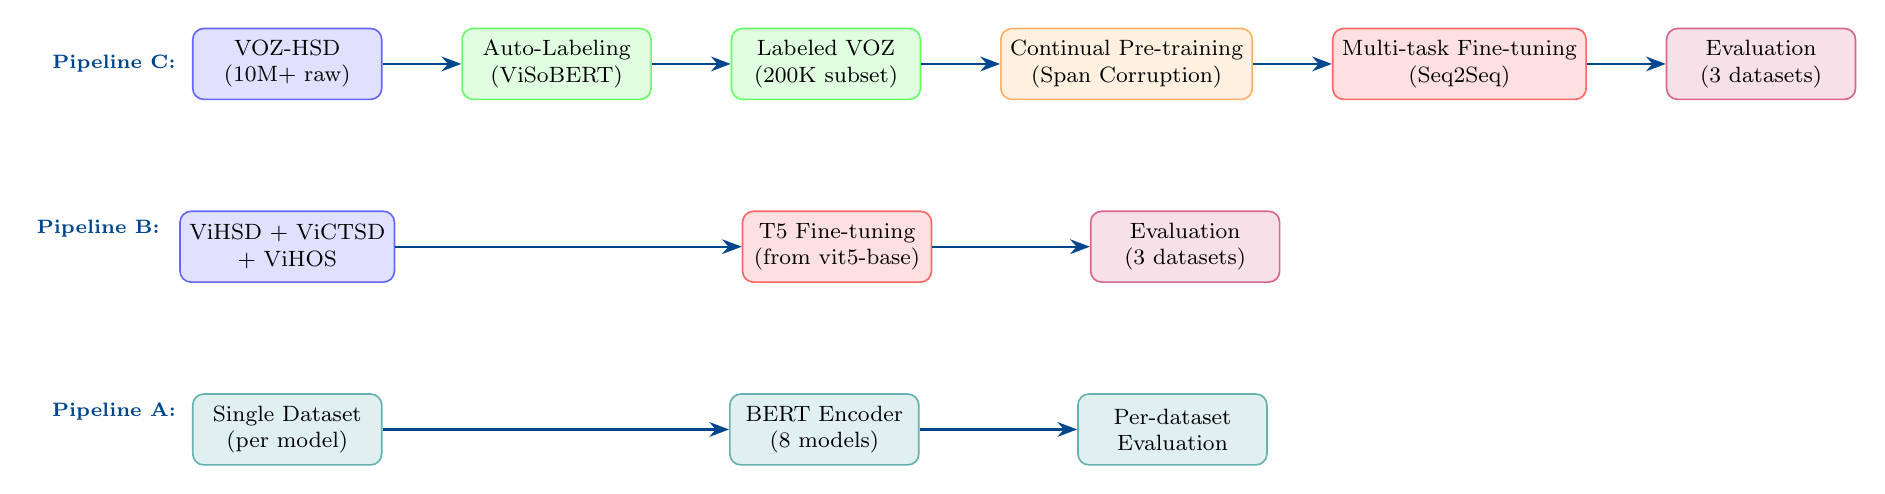
\begin{tikzpicture}[node distance=0.8cm and 1.0cm]
      % === Pipeline C: Data-Centric (top row) ===
      \node[mylbl] at (-2.2, 0) {Pipeline C:};
      \node[pipelinebox=blue] (voz) {VOZ-HSD\\(10M+ raw)};
      \node[pipelinebox=green, right=of voz] (autolabel) {Auto-Labeling\\(ViSoBERT)};
      \node[pipelinebox=green, right=of autolabel] (labeled) {Labeled VOZ\\(200K subset)};
      \node[pipelinebox=orange, right=of labeled] (pretrain) {Continual Pre-training\\(Span Corruption)};
      \node[pipelinebox=red, right=of pretrain] (finetune) {Multi-task Fine-tuning\\(Seq2Seq)};
      \node[pipelinebox=purple, right=of finetune] (eval) {Evaluation\\(3 datasets)};

      % Arrows top row
      \draw[myarrow] (voz) -- (autolabel);
      \draw[myarrow] (autolabel) -- (labeled);
      \draw[myarrow] (labeled) -- (pretrain);
      \draw[myarrow] (pretrain) -- (finetune);
      \draw[myarrow] (finetune) -- (eval);

      % === Pipeline B: T5 without pre-training (middle) ===
      \node[mylbl, below=1.4cm of voz, xshift=-2.4cm] {Pipeline B:};
      \node[pipelinebox=blue, below=1.4cm of voz] (datasets) {ViHSD + ViCTSD\\+ ViHOS};
      \node[pipelinebox=red, right=of datasets, xshift=3.4cm] (t5ft) {T5 Fine-tuning\\(from vit5-base)};
      \node[pipelinebox=purple, right=of t5ft, xshift=1.0cm] (t5eval) {Evaluation\\(3 datasets)};

      \draw[myarrow] (datasets) -- (t5ft);
      \draw[myarrow] (t5ft) -- (t5eval);

      % === Pipeline A: BERT baselines (bottom) ===
      \node[mylbl, below=1.4cm of datasets, xshift=-2.2cm] {Pipeline A:};
      \node[pipelinebox=teal, below=1.4cm of datasets] (bertdata) {Single Dataset\\(per model)};
      \node[pipelinebox=teal, right=of bertdata, xshift=3.4cm] (bert) {BERT Encoder\\(8 models)};
      \node[pipelinebox=teal, right=of bert, xshift=1.0cm] (berteval) {Per-dataset\\Evaluation};

      \draw[myarrow] (bertdata) -- (bert);
      \draw[myarrow] (bert) -- (berteval);
    \end{tikzpicture}
    }%
  \end{center}
  \vspace{0.1cm}
  \begin{itemize}
    \item \textbf{Pipeline A}: BERT baselines (8 encoders, per-dataset)
    \item \textbf{Pipeline B}: T5 text-to-text (ViHateT5, multi-task)
    \item \textbf{Pipeline C}: Data-centric improvement (auto-label $\rightarrow$ pre-train $\rightarrow$ fine-tune)
  \end{itemize}
\end{frame}

% ----------------------------------------------------------
\begin{frame}[shrink=10]{Approach 1: BERT-based Classification (Baseline)}
  \begin{columns}[T]
    \column{0.48\textwidth}
    \begin{block}{Architecture}
      \begin{itemize}
        \item Standard encoder-only transformers
        \item Pre-trained encoder + classification head
        \item Fine-tuned \textbf{independently} on each dataset
      \end{itemize}
    \end{block}
    \vspace{0.2cm}
    \begin{exampleblock}{Models Evaluated}
      \begin{itemize}
        \item \textbf{PhoBERT} (base, v2, large)
        \item \textbf{ViSoBERT} (best performer)
        \item \textbf{XLM-RoBERTa} (base, large)
        \item \textbf{BERT} (multilingual cased/uncased)
        \item \textbf{DistilBERT}, \textbf{viBERT}
      \end{itemize}
    \end{exampleblock}

    \column{0.48\textwidth}
    \begin{block}{Training Configuration}
      \begin{itemize}
        \item Batch size: 16
        \item Learning rate: $2 \times 10^{-5}$
        \item Epochs: 10
        \item Early stopping: patience = 3
        \item Optimizer: AdamW
        \item Max length: 256 tokens
      \end{itemize}
    \end{block}
    \vspace{0.2cm}
    \begin{center}
      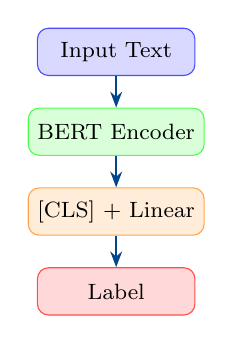
\begin{tikzpicture}
        \node[bertbox=blue] (input) {Input Text};
        \node[bertbox=green, below=0.4cm of input] (enc) {BERT Encoder};
        \node[bertbox=orange, below=0.4cm of enc] (cls) {[CLS] + Linear};
        \node[bertbox=red, below=0.4cm of cls] (out) {Label};
        \draw[myarrow2] (input) -- (enc);
        \draw[myarrow2] (enc) -- (cls);
        \draw[myarrow2] (cls) -- (out);
      \end{tikzpicture}
    \end{center}
  \end{columns}
\end{frame}

% ----------------------------------------------------------
\begin{frame}[shrink=8]{Approach 2: T5 Text-to-Text (ViHateT5)}
  \begin{columns}[T]
    \column{0.50\textwidth}
    \begin{block}{Text-to-Text Formulation}
      All tasks are formulated as sequence-to-sequence:
      \begin{itemize}
        \item \textbf{ViHSD}: \texttt{hate-speech-detection: <text>}\\
              $\rightarrow$ \texttt{CLEAN} / \texttt{OFFENSIVE} / \texttt{HATE}
        \item \textbf{ViCTSD}: \texttt{toxic-speech-detection: <text>}\\
              $\rightarrow$ \texttt{NONE} / \texttt{TOXIC}
        \item \textbf{ViHOS}: \texttt{hate-spans-detection: <text>}\\
              $\rightarrow$ text with \texttt{[HATE]...[HATE]} tags
      \end{itemize}
    \end{block}
    \vspace{0.2cm}
    \begin{exampleblock}{Advantage}
      A \textbf{single model} handles all three tasks via task-specific prefixes --- no need for separate classifiers.
    \end{exampleblock}

    \column{0.46\textwidth}
    \begin{block}{Training Configuration}
      \begin{itemize}
        \item Base model: \textbf{VietAI/vit5-base}
        \item Batch size: 32
        \item Learning rate: $2 \times 10^{-4}$
        \item Epochs: 4
        \item Weight decay: 0.01
        \item Best model metric: Macro F1
        \item Mixed precision: bf16
      \end{itemize}
    \end{block}
    \vspace{0.2cm}
    \begin{block}{Multi-task Training}
      All three datasets are \textbf{concatenated} and trained \textbf{jointly} in a single run. Evaluation is performed per-dataset.
    \end{block}
  \end{columns}
\end{frame}

% ----------------------------------------------------------
\begin{frame}[shrink=12]{Approach 3: Data-Centric Improvement}
  \begin{block}{Key Innovation Beyond Original Paper}
    Auto-labeling + continual pre-training on large-scale domain data before fine-tuning.
  \end{block}
  \vspace{0.2cm}

  \begin{columns}[T]
    \column{0.32\textwidth}
    \begin{block}{\small Step 1: Auto-Labeling}
      \begin{itemize}
        \item Fine-tuned \textbf{ViSoBERT} labels 10M+ VOZ comments
        \item 97.5\% agreement with manual labels
        \item Batch inference on H200 GPU
      \end{itemize}
    \end{block}

    \column{0.32\textwidth}
    \begin{block}{\small Step 2: Pre-training}
      \begin{itemize}
        \item \textbf{Span Corruption} objective on labeled VOZ data
        \item Two setups:
          \begin{itemize}
            \item 100K hate-only
            \item 200K balanced
          \end{itemize}
        \item 10 epochs, lr = $5 \times 10^{-3}$
      \end{itemize}
    \end{block}

    \column{0.32\textwidth}
    \begin{block}{\small Step 3: Fine-tuning}
      \begin{itemize}
        \item Fine-tune from \textbf{domain checkpoint}
        \item Same multi-task Seq2Seq setup
        \item Improved contextual understanding
      \end{itemize}
    \end{block}
  \end{columns}

  \vspace{0.3cm}
  \begin{center}
    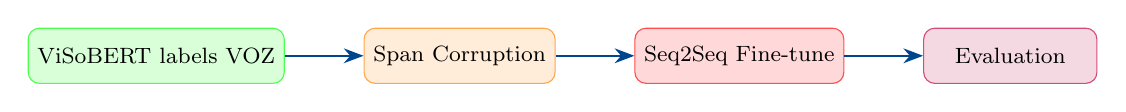
\begin{tikzpicture}
      \node[dcbox=green] (s1) {ViSoBERT labels VOZ};
      \node[dcbox=orange, right=1cm of s1] (s2) {Span Corruption};
      \node[dcbox=red, right=1cm of s2] (s3) {Seq2Seq Fine-tune};
      \node[dcbox=purple, right=1cm of s3] (s4) {Evaluation};
      \draw[myarrow] (s1) -- (s2);
      \draw[myarrow] (s2) -- (s3);
      \draw[myarrow] (s3) -- (s4);
    \end{tikzpicture}
  \end{center}
\end{frame}

% ----------------------------------------------------------
\begin{frame}[shrink=8]{Span Corruption Pre-training}
  \begin{columns}[T]
    \column{0.50\textwidth}
    \begin{block}{How Span Corruption Works}
      \begin{enumerate}
        \item Randomly select \textbf{15\%} of tokens as noise
        \item Replace consecutive corrupted tokens with \textbf{sentinel tokens} (\texttt{<extra\_id\_0>}, \texttt{<extra\_id\_1>}, \ldots)
        \item Model learns to \textbf{predict the original spans}
        \item Mean noise span length: 3.0 tokens
      \end{enumerate}
    \end{block}
    \vspace{0.2cm}
    \begin{exampleblock}{Example}
      \textbf{Input}: ``\texttt{Tôi \textcolor{red}{<extra\_id\_0>} Việt Nam \textcolor{red}{<extra\_id\_1>}}''\\[3pt]
      \textbf{Target}: ``\texttt{\textcolor{red}{<extra\_id\_0>} yêu \textcolor{red}{<extra\_id\_1>} rất nhiều}''
    \end{exampleblock}

    \column{0.46\textwidth}
    \begin{block}{Pre-training Configuration}
      \begin{itemize}
        \item Model: \textbf{VietAI/vit5-base}
        \item Noise density: 0.15
        \item Mean span length: 3.0
        \item Batch size: 128
        \item Learning rate: $5 \times 10^{-3}$
        \item Epochs: 10
        \item Warmup steps: 2000
        \item Optimizer: AdamW
        \item Gradient checkpointing: enabled
        \item Mixed precision: bf16
      \end{itemize}
    \end{block}
  \end{columns}
\end{frame}

% ============================================================
\section{Experiments}
% ============================================================

\begin{frame}[shrink=5]{Training Configurations Summary}
  \begin{table}[h]
    \centering
    \resizebox{0.92\textwidth}{!}{%
    \begin{tabular}{lccccl}
      \toprule
      \textbf{Stage} & \textbf{Base Model} & \textbf{Batch Size} & \textbf{LR} & \textbf{Epochs} & \textbf{Optimizer} \\
      \midrule
      Pre-training T5    & vit5-base              & 128 & $5 \times 10^{-3}$ & 10 & AdamW \\
      Fine-tuning T5     & Pre-trained checkpoint & 32  & $2 \times 10^{-4}$ & 4  & AdamW \\
      Training BERT      & phobert / visobert     & 16  & $2 \times 10^{-5}$ & 10 & AdamW \\
      Auto-Labeling      & visobert (fine-tuned)   & 128 & ---                & ---& --- \\
      \bottomrule
    \end{tabular}}
    \caption{Training configurations for all stages}
  \end{table}

  \vspace{0.2cm}
  \begin{columns}[T]
    \column{0.48\textwidth}
    \begin{block}{Hardware}
      \begin{itemize}
        \item \textbf{NVIDIA H200} (141 GB) -- Pre-training \& auto-labeling
        \item \textbf{P100} -- BERT fine-tuning
        \item GPU provided by FPT via voucher
      \end{itemize}
    \end{block}

    \column{0.48\textwidth}
    \begin{block}{Reproducibility}
      \begin{itemize}
        \item All scripts in \texttt{scripts/} directory
        \item Configurable CLI arguments
        \item Random seed: 42
        \item Models \& data on HuggingFace
      \end{itemize}
    \end{block}
  \end{columns}
\end{frame}

% ============================================================
\section{Results}
% ============================================================

\begin{frame}[shrink=5]{Auto-Labeling Performance}
  \begin{columns}[T]
    \column{0.45\textwidth}
    \begin{block}{ViSoBERT Auto-Labeling}
      \begin{table}[h]
        \centering
        \begin{tabular}{lr}
          \toprule
          \textbf{Metric} & \textbf{Result} \\
          \midrule
          Total samples labeled & 10,747,733 \\
          Agreement w/ manual   & \textbf{97.5\%} \\
          Accuracy              & 97.5\% \\
          Hardware               & H200 GPU \\
          \bottomrule
        \end{tabular}
      \end{table}
    \end{block}

    \column{0.52\textwidth}
    \begin{exampleblock}{Significance}
      \begin{itemize}
        \item ViSoBERT achieves \textbf{97.5\% accuracy} compared to original manual labels
        \item Enables large-scale pre-training without manual annotation
        \item Two pre-training subsets created:
          \begin{itemize}
            \item \textbf{100K} hate-only samples
            \item \textbf{200K} balanced samples
          \end{itemize}
        \item Dataset published on HuggingFace
      \end{itemize}
    \end{exampleblock}
  \end{columns}
\end{frame}

% ----------------------------------------------------------
\begin{frame}[shrink=5]{BERT Results -- Per Dataset (Table 3)}
  \begin{columns}[T]
    \column{0.32\textwidth}
    \begin{block}{\small ViHSD}
      \resizebox{\textwidth}{!}{%
      \begin{tabular}{lcc}
        \toprule
        \textbf{Model} & \textbf{Acc} & \textbf{F1} \\
        \midrule
        \textbf{ViSoBERT}   & .8842 & \textbf{.6871} \\
        PhoBERT v2           & .8725 & .6583 \\
        XLM-R                & .8692 & .6544 \\
        BERT (cased)         & .8665 & .6427 \\
        PhoBERT              & .8632 & .6360 \\
        DistilBERT           & .8615 & .6224 \\
        BERT (uncased)       & .8561 & .6161 \\
        viBERT               & .8596 & .6149 \\
        \bottomrule
      \end{tabular}}
    \end{block}

    \column{0.32\textwidth}
    \begin{block}{\small ViCTSD}
      \resizebox{\textwidth}{!}{%
      \begin{tabular}{lcc}
        \toprule
        \textbf{Model} & \textbf{Acc} & \textbf{F1} \\
        \midrule
        PhoBERT              & .9078 & .7131 \\
        XLM-R                & .9015 & \textbf{.7153} \\
        PhoBERT v2           & .9023 & .7139 \\
        \textbf{ViSoBERT}    & .9035 & .7045 \\
        DistilBERT           & .8962 & .6850 \\
        BERT (uncased)       & .8993 & .6796 \\
        BERT (cased)         & .8983 & .6710 \\
        viBERT               & .8881 & .6765 \\
        \bottomrule
      \end{tabular}}
    \end{block}

    \column{0.32\textwidth}
    \begin{block}{\small ViHOS}
      \resizebox{\textwidth}{!}{%
      \begin{tabular}{lcc}
        \toprule
        \textbf{Model} & \textbf{Acc} & \textbf{F1} \\
        \midrule
        \textbf{ViSoBERT}    & .9016 & \textbf{.8578} \\
        XLM-R                & .8834 & .8133 \\
        BERT (cased)         & .8601 & .7637 \\
        DistilBERT           & .8585 & .7615 \\
        BERT (uncased)       & .8520 & .7393 \\
        PhoBERT v2           & .8492 & .7351 \\
        viBERT               & .8463 & .7291 \\
        PhoBERT              & .8465 & .7281 \\
        \bottomrule
      \end{tabular}}
    \end{block}
  \end{columns}
  \vspace{0.3cm}
  \begin{center}
    \textbf{ViSoBERT} achieves the best average Macro F1 = \textbf{0.7498} across all three datasets.
  \end{center}
\end{frame}

% ----------------------------------------------------------
\begin{frame}[shrink=5]{BERT Average Macro F1 Comparison}
  \begin{table}[h]
    \centering
    \resizebox{0.85\textwidth}{!}{%
    \begin{tabular}{lcccc}
      \toprule
      \textbf{Model} & \textbf{ViHSD F1} & \textbf{ViCTSD F1} & \textbf{ViHOS F1} & \textbf{Avg F1} \\
      \midrule
      \rowcolor{uitlightblue} \textbf{ViSoBERT}     & 0.6871 & 0.7045 & 0.8578 & \textbf{0.7498} \\
      XLM-RoBERTa                                     & 0.6544 & 0.7153 & 0.8133 & 0.7277 \\
      PhoBERT v2                                       & 0.6583 & 0.7139 & 0.7351 & 0.7024 \\
      BERT (cased)                                     & 0.6427 & 0.6710 & 0.7637 & 0.6925 \\
      PhoBERT                                          & 0.6360 & 0.7131 & 0.7281 & 0.6924 \\
      DistilBERT                                       & 0.6224 & 0.6850 & 0.7615 & 0.6896 \\
      BERT (uncased)                                   & 0.6161 & 0.6796 & 0.7393 & 0.6783 \\
      viBERT                                           & 0.6149 & 0.6765 & 0.7291 & 0.6735 \\
      \midrule
      \textbf{Overall Average}                         & 0.6412 & 0.6949 & 0.7660 & 0.7007 \\
      \bottomrule
    \end{tabular}}
    \caption{Average Macro F1 across 3 datasets (Table 3)}
  \end{table}
\end{frame}

% ----------------------------------------------------------
\begin{frame}[shrink=10]{T5 Models -- Detailed Results (Table 4)}
  \begin{table}[h]
    \centering
    \resizebox{0.95\textwidth}{!}{%
    \begin{tabular}{llccc}
      \toprule
      \textbf{Model} & \textbf{Dataset} & \textbf{Accuracy} & \textbf{F1 Weighted} & \textbf{F1 Macro} \\
      \midrule
      ViT5 (Base) & ViHSD  & 0.8777 & 0.8787 & 0.6625 \\
      ViT5 (Base) & ViCTSD & 0.9080 & 0.9178 & 0.7163 \\
      ViT5 (Base) & ViHOS  & 0.9075 & 0.9000 & 0.8612 \\
      \midrule
      mT5 (Base) & ViHSD  & 0.8746 & 0.8877 & 0.6246 \\
      mT5 (Base) & ViCTSD & 0.8932 & 0.9024 & 0.7053 \\
      mT5 (Base) & ViHOS  & 0.9075 & 0.8957 & 0.8501 \\
      \midrule
      \rowcolor{uitlightblue} \textbf{ViHateT5 (Ours)} & ViHSD  & \textbf{0.8815} & \textbf{0.8849} & \textbf{0.6698} \\
      \rowcolor{uitlightblue} \textbf{ViHateT5 (Ours)} & ViCTSD & \textbf{0.9105} & \textbf{0.9158} & \textbf{0.7189} \\
      \rowcolor{uitlightblue} \textbf{ViHateT5 (Ours)} & ViHOS  & \textbf{0.9081} & \textbf{0.9055} & \textbf{0.8616} \\
      \bottomrule
    \end{tabular}}
    \caption{T5 model comparison (Table 4 -- Paper Reproduction)}
  \end{table}

  \vspace{0.2cm}
  \begin{table}[h]
    \centering
    \begin{tabular}{lcccc}
      \toprule
      \textbf{Model} & \textbf{ViHSD} & \textbf{ViCTSD} & \textbf{ViHOS} & \textbf{Avg F1} \\
      \midrule
      \rowcolor{uitlightblue} \textbf{ViHateT5 (Ours)} & \textbf{0.6698} & \textbf{0.7189} & \textbf{0.8616} & \textbf{0.7501} \\
      ViT5 (Base) & 0.6625 & 0.7163 & 0.8612 & 0.7467 \\
      mT5 (Base) & 0.6246 & 0.7053 & 0.8501 & 0.7267 \\
      \bottomrule
    \end{tabular}
    \caption{Average Macro F1 for T5 models}
  \end{table}
\end{frame}

% ----------------------------------------------------------
\begin{frame}[shrink=12]{Pre-training Impact (Table 5)}
  \begin{columns}[T]
    \column{0.48\textwidth}
    \begin{block}{100K Hate-Only Pre-training}
      \begin{table}[h]
        \centering
        \resizebox{\textwidth}{!}{%
        \begin{tabular}{lccc}
          \toprule
          \textbf{Dataset} & \textbf{Acc} & \textbf{F1-W} & \textbf{F1-M} \\
          \midrule
          ViHSD  & 0.8789 & 0.8784 & 0.6808 \\
          ViCTSD & 0.9070 & 0.9283 & 0.6586 \\
          ViHOS  & 0.9039 & 0.8981 & 0.8541 \\
          \bottomrule
        \end{tabular}}
      \end{table}
    \end{block}

    \column{0.48\textwidth}
    \begin{block}{200K Balanced Pre-training}
      \begin{table}[h]
        \centering
        \resizebox{\textwidth}{!}{%
        \begin{tabular}{lccc}
          \toprule
          \textbf{Dataset} & \textbf{Acc} & \textbf{F1-W} & \textbf{F1-M} \\
          \midrule
          ViHSD  & \textbf{0.8815} & \textbf{0.8849} & 0.6698 \\
          ViCTSD & \textbf{0.9105} & 0.9158 & \textbf{0.7189} \\
          ViHOS  & \textbf{0.9081} & \textbf{0.9055} & \textbf{0.8616} \\
          \bottomrule
        \end{tabular}}
      \end{table}
    \end{block}
  \end{columns}

  \vspace{0.3cm}
  \begin{table}[h]
    \centering
    \begin{tabular}{lcccc}
      \toprule
      \textbf{Pre-training Setup} & \textbf{ViHSD} & \textbf{ViCTSD} & \textbf{ViHOS} & \textbf{Avg F1} \\
      \midrule
      \rowcolor{uitlightblue} \textbf{200K Balanced} & 0.6698 & \textbf{0.7189} & \textbf{0.8616} & \textbf{0.7501} \\
      100K Hate-Only & \textbf{0.6808} & 0.6586 & 0.8541 & 0.7312 \\
      \bottomrule
    \end{tabular}
    \caption{Pre-training impact comparison (Table 5)}
  \end{table}

  \begin{center}
    $\Rightarrow$ \textbf{200K balanced} pre-training yields better overall performance (+1.9\% avg F1).
  \end{center}
\end{frame}

% ----------------------------------------------------------
\begin{frame}[shrink=5]{Extended BERT Comparison (Table 6)}
  \begin{columns}[T]
    \column{0.48\textwidth}
    \begin{block}{Multilingual Models}
      \resizebox{\textwidth}{!}{%
      \begin{tabular}{lccc}
        \toprule
        \textbf{Model} & \textbf{Acc} & \textbf{F1-W} & \textbf{F1-M} \\
        \midrule
        xlm-roberta-large     & 0.9204 & 0.7755 & 0.7968 \\
        xlm-roberta-base      & 0.9189 & 0.7722 & 0.8028 \\
        distilbert-multi      & 0.9115 & 0.7459 & 0.7754 \\
        bert-multi-uncased    & 0.9102 & 0.7557 & 0.7784 \\
        bert-multi-cased      & 0.9094 & 0.7548 & 0.7740 \\
        \bottomrule
      \end{tabular}}
    \end{block}

    \column{0.48\textwidth}
    \begin{block}{Monolingual (Vietnamese) Models}
      \resizebox{\textwidth}{!}{%
      \begin{tabular}{lccc}
        \toprule
        \textbf{Model} & \textbf{Acc} & \textbf{F1-W} & \textbf{F1-M} \\
        \midrule
        \rowcolor{uitlightblue} \textbf{visobert} & \textbf{0.9296} & \textbf{0.8051} & \textbf{0.8128} \\
        phobert-large         & 0.9245 & 0.7895 & 0.7832 \\
        phobert-base-v2       & 0.9216 & 0.7888 & 0.7810 \\
        vibert-base-cased     & 0.9117 & 0.7385 & 0.7771 \\
        phobert-base          & 0.9231 & 0.7562 & 0.7764 \\
        \bottomrule
      \end{tabular}}
    \end{block}
  \end{columns}

  \vspace{0.3cm}
  \begin{exampleblock}{Key Finding}
    \textbf{ViSoBERT} achieves the highest Macro F1 (\textbf{0.8128}) among all 10 BERT variants. Monolingual pre-training on Vietnamese social media data provides a clear advantage.
  \end{exampleblock}
\end{frame}

% ----------------------------------------------------------
\begin{frame}[shrink=5]{Results Summary}
  \begin{block}{Key Findings}
    \begin{enumerate}
      \item \textbf{ViHateT5 (Ours)} achieves the best T5 avg Macro F1 = \textbf{0.7501}, outperforming ViT5 (0.7467) and mT5 (0.7267)
      \item \textbf{200K balanced pre-training} outperforms 100K hate-only (+1.9\% avg F1)
      \item \textbf{ViSoBERT} is the best encoder model (avg F1 = 0.7498, extended F1 = 0.8128)
      \item Auto-labeling achieves \textbf{97.5\% accuracy} on 10.7M samples
    \end{enumerate}
  \end{block}
  \vspace{0.2cm}

  \begin{columns}[T]
    \column{0.48\textwidth}
    \begin{exampleblock}{Best Models Per Task}
      \begin{itemize}
        \item \textbf{ViHSD}: ViHateT5 (F1 = 0.6698)
        \item \textbf{ViCTSD}: ViHateT5 (F1 = 0.7189)
        \item \textbf{ViHOS}: ViHateT5 (F1 = 0.8616)
      \end{itemize}
    \end{exampleblock}

    \column{0.48\textwidth}
    \begin{alertblock}{Observation}
      \begin{itemize}
        \item T5 text-to-text approach slightly edges BERT baselines
        \item Unified model vs.\ 8 separate BERT classifiers
        \item Domain pre-training is more impactful than model size
      \end{itemize}
    \end{alertblock}
  \end{columns}
\end{frame}

% ============================================================
\section{Limitations \& Future Work}
% ============================================================

\begin{frame}[shrink=5]{Limitations \& Future Work}
  \begin{columns}[T]
    \column{0.48\textwidth}
    \begin{alertblock}{Current Limitations}
      \begin{itemize}
        \item Improvement is purely \textbf{data-centric}; model architecture unchanged
        \item Minority classes (e.g., OFFENSIVE in ViHSD) remain challenging
        \item Auto-labeling may \textbf{propagate biases} from ViSoBERT into pre-training data
        \item Limited to Vietnamese language only
      \end{itemize}
    \end{alertblock}

    \column{0.48\textwidth}
    \begin{exampleblock}{Future Directions}
      \begin{itemize}
        \item \textbf{Model-centric improvements}: focal loss, curriculum learning, architecture modifications
        \item Deeper \textbf{error analysis} and failure case studies
        \item \textbf{Data augmentation} for underrepresented classes
        \item Larger pre-training corpus and longer schedules
        \item Cross-lingual transfer for other low-resource languages
      \end{itemize}
    \end{exampleblock}
  \end{columns}
\end{frame}

% ============================================================
\section{Conclusion}
% ============================================================

\begin{frame}[shrink=8]{Conclusion}
  \begin{block}{Summary}
    \begin{itemize}
      \item Successfully \textbf{reimplemented ViHateT5} (ACL 2024) with reproducible results
      \item Built an \textbf{auto-labeling pipeline} (ViSoBERT, 97.5\% accuracy, 10.7M samples)
      \item Demonstrated the value of \textbf{data-centric improvement}: balanced pre-training yields +1.9\% avg F1 over hate-only
      \item Comprehensive benchmarking: \textbf{8 BERT} + \textbf{3 T5} models across \textbf{3 datasets}
      \item All models and datasets published on \textbf{HuggingFace}
    \end{itemize}
  \end{block}
  \vspace{0.3cm}

  \begin{exampleblock}{Resources}
    \begin{itemize}
      \item \textbf{GitHub}: \url{https://github.com/paht2005/DS200.Q21-Group2-Reimplementation-and-Improvement-of-ViHateT5-for-Vietnamese-HSD-Project}
      \item \textbf{HuggingFace}: \url{https://huggingface.co/collections/NCPhat2005/ds200q21-big-data-analysis-group-2}
    \end{itemize}
  \end{exampleblock}

  \vspace{0.3cm}
  \begin{center}
    {\Large\bfseries\color{uitblue} Thank you! Questions?}
  \end{center}
\end{frame}

% ============================================================
\section{References}
% ============================================================

\begin{frame}{References}
  \begin{thebibliography}{9}
    \bibitem{vihatet5}
    Luan Thanh Nguyen,
    \textit{``ViHateT5: Enhancing Hate Speech Detection in Vietnamese With a Unified Text-to-Text Transformer Model,''}
    Findings of ACL 2024, pp.\,5948--5961.

    \bibitem{vit5}
    VietAI,
    \textit{``ViT5: Pretrained Text-to-Text Transformer for Vietnamese Language Generation,''}
    NAACL 2022 (SRW).

    \bibitem{t5}
    C.\,Raffel et al.,
    \textit{``Exploring the Limits of Transfer Learning with a Unified Text-to-Text Transformer,''}
    JMLR, 2020.

    \bibitem{phobert}
    D.\,Q.\,Nguyen and A.\,T.\,Nguyen,
    \textit{``PhoBERT: Pre-trained Language Models for Vietnamese,''}
    Findings of EMNLP 2020.
  \end{thebibliography}
\end{frame}

\end{document}
